\documentclass[10pt,a4paper,final]{article}
\usepackage[utf8]{inputenc}

\usepackage{amsmath}
\usepackage{amsfonts}
\usepackage{amssymb}
\usepackage{wrapfig}
\usepackage{listings}

\usepackage[font=small,labelfont=bf]{caption}
\setlength{\columnsep}{22pt}

\usepackage{parskip}
\usepackage{amsmath}
\usepackage{hyperref}
\usepackage{amssymb}
\usepackage{graphicx}
\usepackage{float}
\restylefloat{figure}

\author{Goette Marcelo}
\title{Trabajo Practico VII}

\begin{document}

\maketitle

\section{Ejercicio 1}
\begin{itemize}
\item[a.] Para este ejercicio se pide hallar la función para graficar los polos y los ceros de los que se encuentran en la figura 1. Cuyas coordenadas polares son (0.95,45º), (0.95,-45º), (0.95,45º) y (0.95,-45º) para los polos y para los ceros (0.80,30º), (0.80,-30º), (0.80,60º) y (0.80,-60º). Entonces, la función seria:

\begin{figure}[h!]
\centering
  \caption{Diagrama de polos y ceros.}
  \label{fig:pyc}
  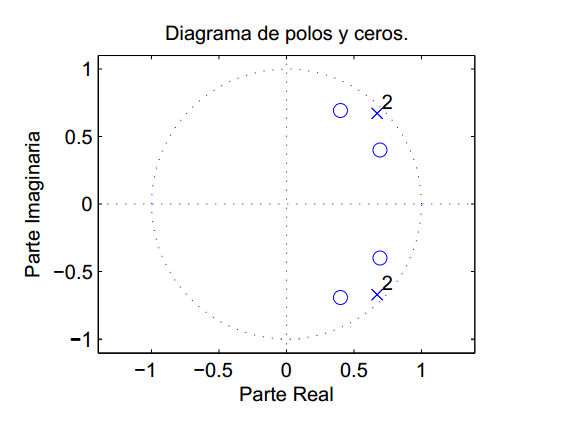
\includegraphics[scale=0.7]{fig1.png}
    
\end{figure}

\begin{lstlisting}
function [c, p] = encontrarRaices(rz, rp)
    p = [rp * (sin(pi/4) + j * cos(pi/4));
        rp * (sin(-pi/4) + j * cos(-pi/4));
        rp * (sin(pi/4) + j * cos(pi/4));
        rp * (sin(-pi/4) + j * cos(-pi/4))];
    
    c = [rz * (sin(pi/6) + j * cos(pi/6));
        rz * (sin(-pi/6) + j * cos(-pi/6));
        rz * (sin(pi/3) + j * cos(pi/3));
        rz * (sin(-pi/3) + j * cos(-pi/3))];

endfunction
\end{lstlisting}
%codigo

\item[b.] Para poder graficar la respuesta en frecuencia del filtro entre 0 y $\pi$ tenemos que primero hallar el polinomio $H(z)$ con los polos y ceros.

\begin{lstlisting}
function [xz, yz] = polinomioH(zeros, polos)
    lz = length(zeros);
    lp = length(polos);
    xz = [1];
    yz = [1];
    for i=1:lp
        yz = conv(yz, [1 -polos(i)]);
    end
    for i=1:lz
        xz = conv(xz, [1 -zeros(i)]);
    end
    
end
\end{lstlisting}
%codigo
Para obtener la respuesta en frecuencia, utilizaremos la función freqz, que evaluará a $H(z)$ en un circulo unitario $z = e^{j\theta}$ con una frecuencia de muestreo $f_m$.

\begin{lstlisting}
fm = 200;
[num, den] = polinomioH(c,p);
resp_frec = freqz(num, den, fm);
\end{lstlisting}

\begin{figure}[h!]
\centering
  \caption{Respuesta en frecuencia.}
  \label{fig:resp}
  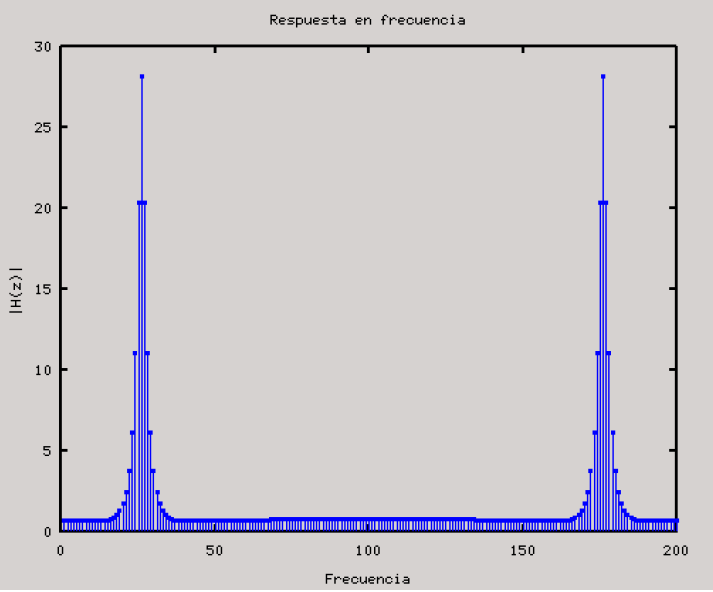
\includegraphics[scale=0.4]{fig2.png}
    
\end{figure}

En la figura 2, se observa que el fitro es un pasa-banda de 25 Hz. para señales muestreadas a 200 Hz.

\item[c.] Para normalizar los coeficientes de filtro primeros se calculara un factor de normalización que es $N=1/M$ donde $M$ es el máximo valor de la respuesta en frecuencia. Segundo, se calcular $Y_N(z)=N*Y(z)$ con este $Y_N(z)$ se calcula la respuesta en frecuencia normalizada, como se muestra en la figura 3.


\begin{lstlisting}
fact_normlizacion = 1/max(abs(respuesta_freq));
num_norm = num * fact_normalizacion;
resp_frec_norm = freqz(num_norm, den, fm);
\end{lstlisting}
%codigo
\begin{figure}[h!]
\centering
  \caption{Respuesta en frecuencia normalizada.}
  \label{fig:respN}
  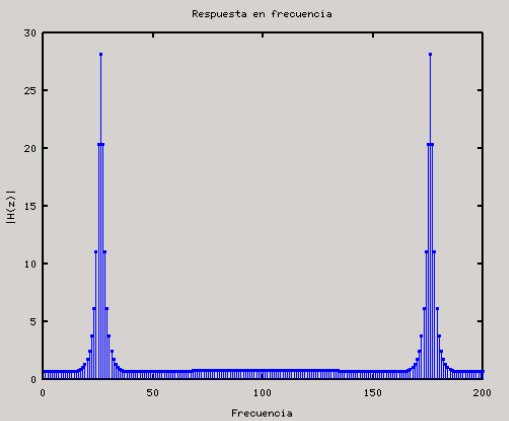
\includegraphics[scale=0.6]{fig3.png}
    
\end{figure}


\item[d.] Al modificar el radio de los, por ejemplo, los pasamos de 0.95 a 0.85 podemos apreciar en las componentes de las frecuencias que antes estaban mas bajas aumentan, figura 4

\begin{figure}[h!]
	\centering
	\caption{Respuesta en frecuencia menor radio.}
  \label{fig:respMenor}
  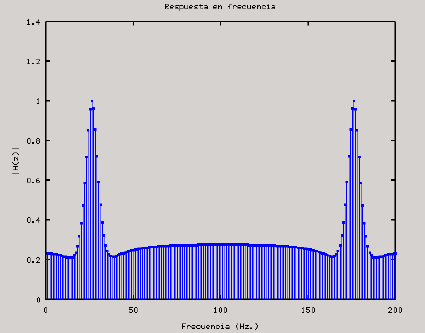
\includegraphics[scale=0.7]{fig4.png}
    
\end{figure}

En el caso anterior vimos cuando disminuíamos el radio, para el caso de aumentarlo a 0.99 podemos ver que el filtro deja pasar frecuencias de 25 Hz. Entonces, este filtro es ideal, pero tiene problemas de estabilidad en el mundo real.

\begin{figure}[h!]
  \centering
  \caption{Respuesta en frecuencia mayor radio.}
  \label{fig:respMayor}
  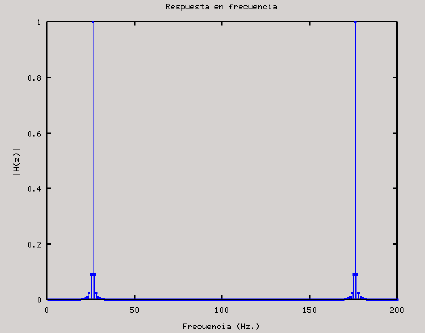
\includegraphics[scale=0.7]{fig5.png}
    
\end{figure}

\item[e.] Ahora probaremos el filtro con una señal de dos senoidales de frecuencia distintas, de 15 Hz y 25 Hz, y muestreadas a 200 Hz.

\begin{lstlisting}
fm = 200;
T = 1/fm;
t = 0 : T : (1-T);

senial = sin(2*pi*t*15) + sin (2*pi*t*25);

espectro = fft(senial);
senial_filtrada = ifft(resp_frec_norm .* espectro');
%plot(real(senial_filtrada));
espectro_filtrado = fft(senial_filtrada);
\end{lstlisting}

%codigo
En la figura 6 se puede observar la señal de prueba y al lado su espectro frecuencial (arriba), se puede ver que tiene frecuencias de 15 y 25 Hz. Después de pasarla por el filtro que tenemos, el espectro de la señal (abajo) pierde la componente frecuencia de 15 Hz y esto tambien se observa en la señal modificada. Con esto podemos ver que el filtro funciono correctamente.

\begin{figure}[h!]
\centering
  \caption{Respuesta en frecuencia de la señal de prueba a 200 Hz.}
  \label{fig:res200}
  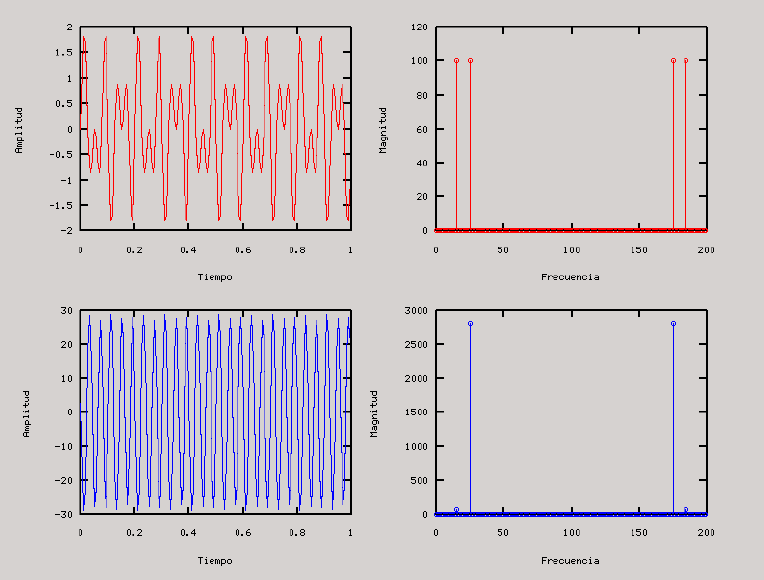
\includegraphics[scale=0.4]{fig6.png}
    
\end{figure}

\item[f.] Ahora probaremos el filtro con la misma señal constituida de dos senoidales de frecuencia distintas, de 15 Hz y 25 Hz, pero ahora muestreadas a 120 Hz.

\begin{figure}[h!]
\centering
  \caption{Respuesta en frecuencia de la señal de prueba a 120 Hz.}
  \label{fig:res120}
  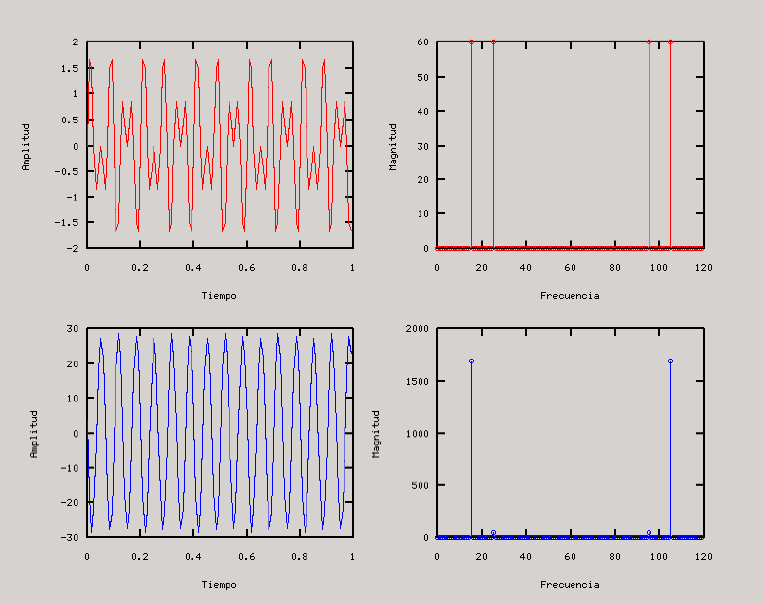
\includegraphics[scale=0.4]{fig7.png}
    
\end{figure}

Se puede ver que ahora el filtro dejo pasar la frecuencia de 15 Hz, esto es porque el filtro es dependiente de la frecuencia de muestreo de a señal de entrada.

\end{itemize}

\section{Ejercicio 2}

\subsection{Filtro Butterworth}
Este tipo de filtros tienen sus ceros en el infinito, ya que, la fórmula del filtro en el plano $S$ para un orden $N$ es:
\[
H_B(s)=\frac{1}{(s-s_1)(s-s_2)...(s-s_{2N})}
\]
podemos ver que tenemos $2N$ polos. Con esto sabemos que la fórmula de los polos es:
\[
s_m=e^{j\pi\frac{(2m+N-1)}{2N}}
\]

para $1\leq m\leq 2N$. Con esto podemos definir un filtro normalizado de orden N mediante la ubicación de sus polos. Pero, para tener un filtro que tenga la frecuencia de paso o rechazo que deseamos, debemos recurrir a maniobras algebraicas.

Entonces, para un filtro pasa-altos con una frecuencia de corte de 500 Hz, vamos a tener que hacerlo de la siguiente manera.

Para cada miembro de $H_B(s)$:
\[ H_{B_i}(s)=\frac{1}{s-s_i} \]
La conversión de filtro pasa-bajos normalizado a  filtro pasa-altos es:
\[ s \rightarrow \frac{w_c}{s} \]
donde $w_c$ es la frecuencia de paso deseada.

Por lo tanto, la ecuación del filtro, luego de reemplazar $s$, queda como:

\[ H_{B_i}(s)=\frac{1}{\frac{w_c}{s}-s_i} \]

\[ H_{B_i}(s)=\frac{s}{w_c-s_is} \]

Para finalizar, multiplicamos numerador y denominador por $\frac{-1}{s_i}$ quedando:

\[ H_{B_i}(s)=\frac{\frac{-s}{s_i}}{s-\frac{w_c}{s_i}} \]

Entonces, para $H_B(s)$  obtenemos la forma general del filtro pasa-altos de Butterworth de orden $N$:

\[ 
H_B(s)=\frac{Gs^{2N}}{(s-\frac{w_c}{s_1})(s-\frac{w_c}{s_2})...(s-\frac{w_c}{s_{2N}})} 
\]
Siendo G la constante de ganancia:
\[
G=\frac{(-1)^{2N}}{s_1s_2...s_{2N}}
\]

Ademas, se puede ver que se agregaron $2N$ ceros en $s=0$ y se generó una constante de ganancia $G$.

Ahora, transformamos el filtro analógico en uno digital aplicándole la transformación bilinial:

\[ s=\frac{2}{T} \frac{1-z^{-1}}{1+z^{-1}} \]

Sin embargo, esta transformada comprime las frecuencias altas a partir de la media del círculo unitario en Z. Para evitar esto aplicamos antes un escalamiento de la frecuencia de corte deseada para evitar este fenómeno:
\[
w_c=\frac{2}{T}tan(\pi wT)
\]
donde $T$ será el período de muestreo de $w$ serán de 500 Hz que son los necesarios para el ejercicio. Y la frecuencia de muestreo elegida es de 2000 Hz, $w_c=4000$.

\begin{lstlisting}
function [sm] = polosButterworh(N)
    
    sm = zeros(1,2*N);
    for i = 1 : 2*N
        sm(i) = exp(j*pi*(N++2*i-1)/(2*N));
    end
    
end

function [nceros, npolos, nganancia] = pasabajo_pasaalto(polos, ganancia, wp)
    nceros = [];
    npolos = [];
    nganancia = ganancia;
    N = length(polos);
    for i=1:N
        polo = polos(i);
        nceros = [nceros 0];
        npolos = [npolos wp/polo];
        nganancia = nganancia * (-1/polo);
    end
end

function zev = evaluarZeta(z, T, polos, ceros, ganancia)
    zev = ganancia;
    s = (2/T) * (1 - z^(-1))/(1 + z^(-1));
    for c = ceros
        zev = zev * (s - c);
    end
    for p = polos
        zev = zev/(s - p);
    end
end

function resp = pasaAltoButterworth(frec_paso, frec_muestreo, orden)
    polos = polosButterworth(orden);
    ganancia = 1;
    T = 1/frec_muestreo;
    w_nueva = (2/T) * tan(pi * frec_paso * T);
    [ceros, polos, ganacia] = pasabajo_pasaalto(polos, ganancia, w_nueva);
    valores = [0:T: (1-T)];
    z = exp(j * 2 * pi * valores);
    for i = 1:length(z);
        resp(i) = evaluarZeta(z(i), T, polos, ceros, ganancia);
    end
end

frec_paso = 500;
frec_muestreo = 2000;
orden = 10;
resp_frec = pasaAltosButterworth( frec_paso , frec_muestreo , orden ) ;
\end{lstlisting}
%codigo

\begin{figure}[h!]
\centering
  \caption{Filtro Butterworth orden 10.}
  \label{fig:res120}
  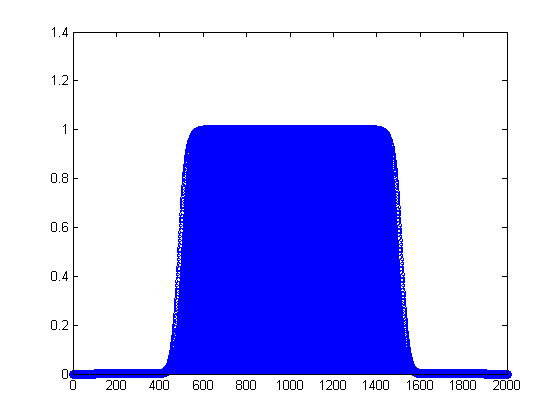
\includegraphics[scale=0.5]{fig8.png}
    
\end{figure}

\begin{figure}[h!]
\centering
  \caption{Filtro Butterworth orden 1.}
  \label{fig:res120}
  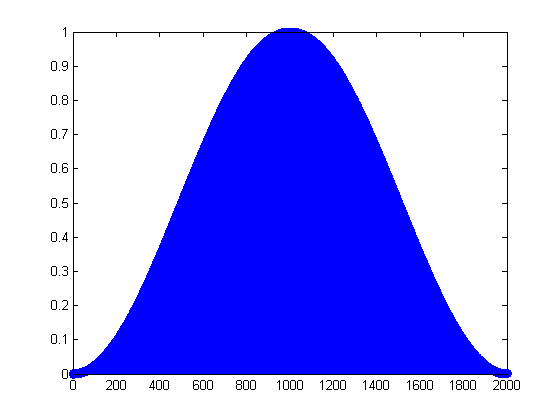
\includegraphics[scale=0.5]{fig9.png}
    
\end{figure}

\begin{figure}[h!]
\centering
  \caption{Filtro Butterworth orden 5.}
  \label{fig:res120}
  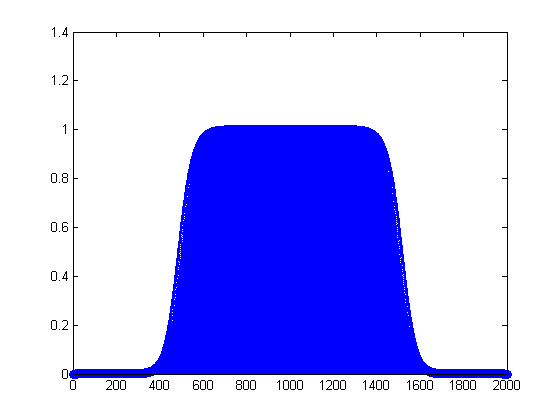
\includegraphics[scale=0.5]{fig10.png}
    
\end{figure}

\begin{figure}[h!]
\centering
  \caption{Filtro Butterworth orden 20.}
  \label{fig:res120}
  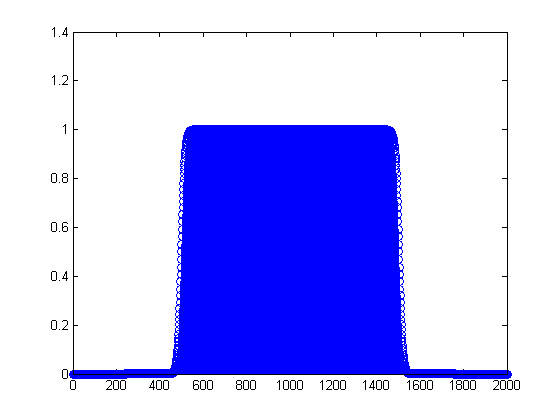
\includegraphics[scale=0.5]{fig11.png}
    
\end{figure}

Como se ven en las figuras 8, 9 ,10 y 11, a medida de que el orden aumenta la banda de transición se vuelve mas chica y se hace mas preciso el filtro.

\section{Ejercicio 3}
Los siguientes filtros son pasa-banda con frecuencia de corte de 2500 y 3000 Hz, con una atenuación máxima en la banda de paso es de 0.7 dB y la atenuación mínima en la banda de rechazo es de 55 dB. También, las banda de transición no es superior a 200 Hz y la frecuencia de muestreo de las señales que procesa es de 10 kHz.

Los filtros que haremos son los de Butterworth, Chebyshev I y II, y el filtro elíptico. Para hacerlos utilizaremos funciones predefinidas de matlab.

\begin{lstlisting}
%Datos
fm = 10000;
fmax = fm/2;
f1 = 2500;
f2 = 3000;
delta = 200;
at_max = 0.7;
at_min = 55;

%Filtro de Butterworth
[butter_n, butterW] = buttord([f1/fmax f2/fmax], [(f1-delta)/fmax (f2+delta)/fmax], at_max, at_min);
[butter_b, butter_a] = butter(ceil(butter_n/2), butterW);

%Filtro de Chebyshev I
[cheby1_n, cheby1_w] = cheb1ord([f1/fmax f2/fmax], [(f1-delta)/fmax (f2+delta)/fmax], at_max, at_min);
[cheby1_b, cheby1_a] = cheby1(cheby1_n, at_max, cheby1_w);

%Filtro de Chebyshev II
[cheby2_n, cheby2_w] = cheb2ord([f1/fmax f2/fmax], [(f1-delta)/fmax (f2+delta)/fmax], at_max, at_min);
[cheby2_b, cheby2_a] = cheby2(cheby2_n, at_min, cheby2_w);

%Filtro eliptico
[elip_n, elip_w] = ellipord([f1/fmax f2/fmax], [(f1-delta)/fmax (f2+delta)/fmax], at_max, at_min);
[elip_b, elip_a] = ellip(elip_n, at_max, at_min, elip_w);

\end{lstlisting}

Sus espectros respectivamente son:
\begin{figure}[h!]
\centering
  \caption{Filtro Butterworth orden 13.}
  \label{fig:res120}
  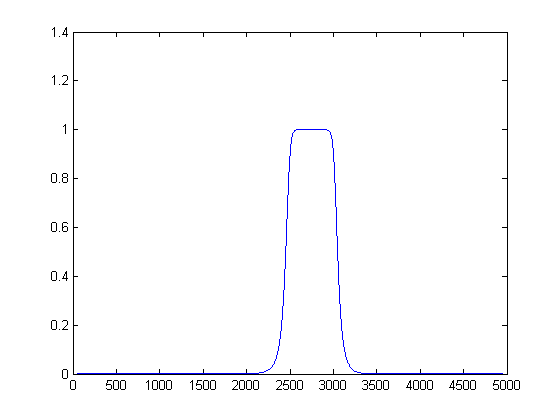
\includegraphics[scale=0.5]{fig12.png}
    
\end{figure}

\begin{figure}[h!]
\centering
  \caption{Filtro Chebyshev tipo I de orden 7.}
  \label{fig:res120}
  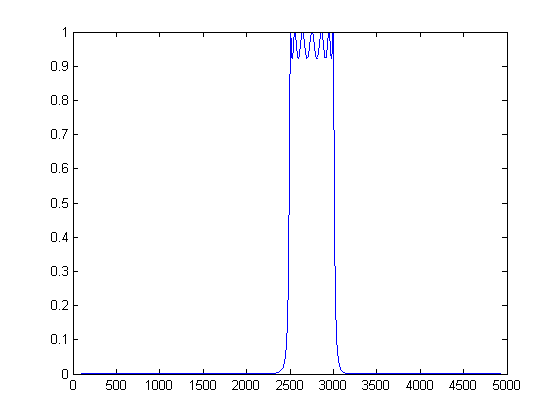
\includegraphics[scale=0.5]{fig13.png}
    
\end{figure}

\begin{figure}[h!]
\centering
  \caption{Filtro Chebyshev tipo II de orden 7.}
  \label{fig:res120}
  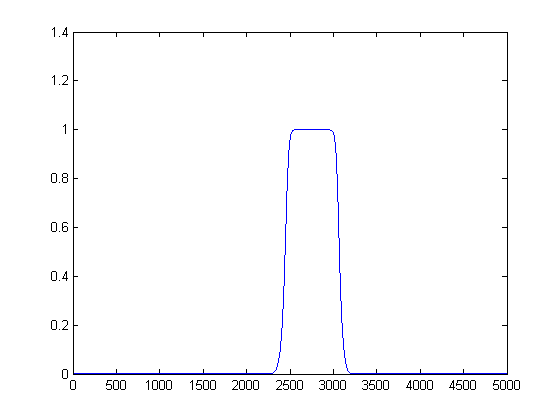
\includegraphics[scale=0.5]{fig14.png}
    
\end{figure}

\begin{figure}[h!]
\centering
  \caption{Filtro Elíptico de orden 5.}
  \label{fig:res120}
  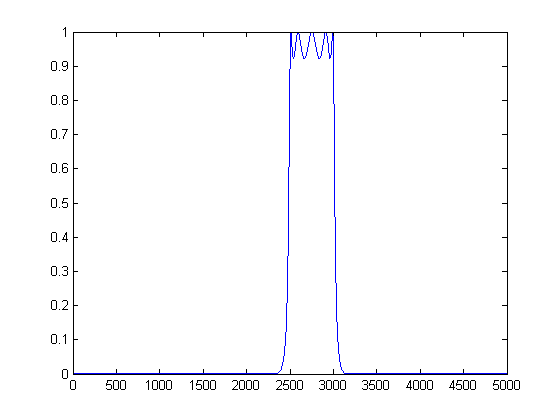
\includegraphics[scale=0.5]{fig15.png}
    
\end{figure}

El filtro que utiliza el menor orden es el filtro elíptico con orden de 5. A continuación, calcularemos los filtros de los demás con un orden de 5:

\begin{figure}[h!]
\centering
  \caption{Filtro Butterworth orden 5.}
  \label{fig:res120}
  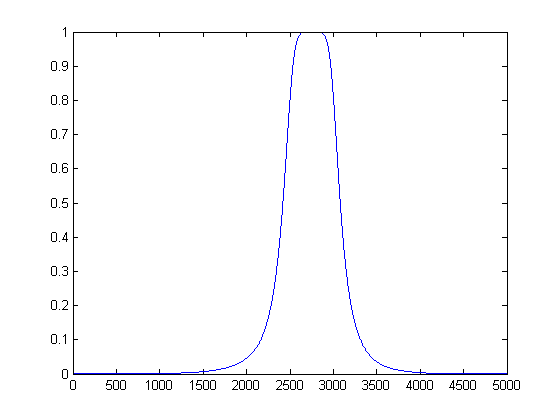
\includegraphics[scale=0.5]{fig16.png}
    
\end{figure}

\begin{figure}[h!]
\centering
  \caption{Filtro Chebyshev tipo I orden 5.}
  \label{fig:res120}
  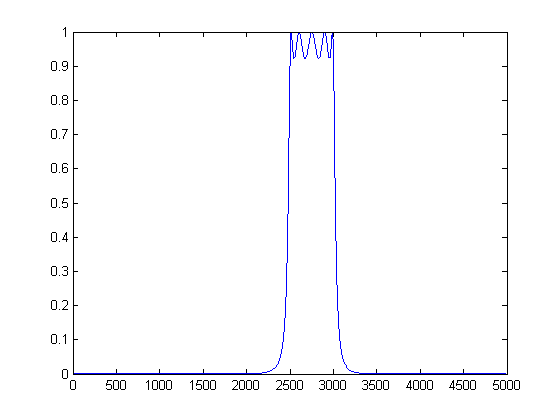
\includegraphics[scale=0.5]{fig17.png}
    
\end{figure}

\begin{figure}[h!]
\centering
  \caption{Filtro Chebyshev tipo II orden 5.}
  \label{fig:res120}
  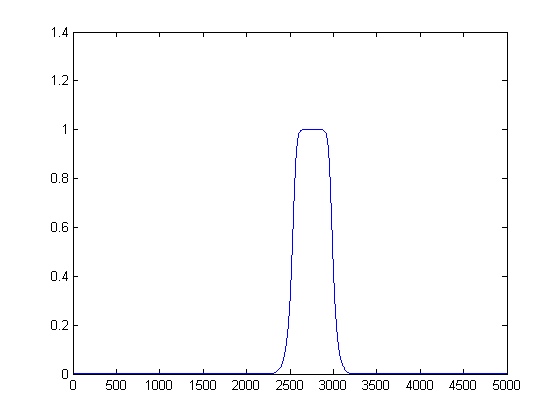
\includegraphics[scale=0.5]{fig18.png}
    
\end{figure}

Se puede observar que los filtros de Chebyshev no varían mucho debido a que su orden anterior era de 7, a diferencia el de butterworth cuyo orden es de 13 la diferencia es notable.

\section{Ejercicio 4}



\end{document}